\documentclass[10pt,aspectratio=169]{beamer}
%\documentclass[12pt,aspectratio=169]{beamer}

%\mode<presentation>

\usepackage{graphicx}
\usepackage{breqn}
\usepackage{bm}
\usepackage{color}
\usepackage{tabularx}

\usepackage{listings}
\lstset{language=C++}

\usepackage{mathtools}
\DeclarePairedDelimiter\ceil{\lceil}{\rceil}
\DeclarePairedDelimiter\floor{\lfloor}{\rfloor}


%\ifxetex
\usepackage{fontspec}
\newfontfamily{\klavikumfont}{Klavika-Regular.otf}
\selectfont\klavikumfont
%\fi


\usepackage{listings}

%\usepackage[utf8]{inputenc}
\definecolor{bluekeywords}{rgb}{0.63, 0.79, 0.95}
\definecolor{greencomments}{rgb}{0,0.5,0}
\definecolor{redstrings}{rgb}{0.64,0.08,0.08}
\definecolor{xmlcomments}{rgb}{0.5,0.5,0.5}
\definecolor{types}{rgb}{0.17,0.57,0.68}
\lstset{language=C++,
captionpos=b,
%numbers=left,
%numberstyle=\tiny,
frame=single,
showspaces=false,
showtabs=false,
breaklines=true,
showstringspaces=false,
breakatwhitespace=true,
escapeinside={(*@}{@*)},
commentstyle=\color{greencomments},
morekeywords={partial, var, value, get, set},
keywordstyle=\color{bluekeywords},
stringstyle=\color{redstrings},
basicstyle=\ttfamily\small,
}

\usepackage[yyyymmdd]{datetime}
\renewcommand{\dateseparator}{-}

%\usepackage[inline]{asymptote}
\usepackage{asymptote}
\def\asylatexdir{}
\def\asydir{}

\renewcommand{\thefootnote}{\fnsymbol{footnote}}

\def\clap#1{\hbox to 0pt{\hss#1\hss}}
\def\mathllap{\mathpalette\mathllapinternal}
\def\mathrlap{\mathpalette\mathrlapinternal}
\def\mathclap{\mathpalette\mathclapinternal}
\def\mathllapinternal#1#2{\llap{$\mathsurround=0pt#1{#2}$}}
\def\mathrlapinternal#1#2{\rlap{$\mathsurround=0pt#1{#2}$}}
\def\mathclapinternal#1#2{\clap{$\mathsurround=0pt#1{#2}$}}

\def\p{\pause}

\def\({\left(}
\def\){\right)}
\def\[{\left[}
\def\]{\right]}

\def\no#1{\nobreak{#1}} % stop equation breaking in dmath

\begin{asydef}
  // Global Asymptote definitions can be put here.
  import three;
  usepackage("bm");
  texpreamble("\def\V#1{\bm{#1}}");
  // One can globally override the default toolbar settings here:
  // settings.toolbar=true;
\end{asydef}

%\useinnertheme{rectangles} %specifies itemize points to be rectangles
\useoutertheme{default}

\definecolor{darkgreen}{RGB}{0, 100, 0}
\definecolor{brightpurple}{RGB}{160,32,240}

% fg specifies foreground color
% bg specifies background color
% the notation color!x!white mixes the color with 1-x amount of white
%\setbeamercolor{frametitle}{fg=darkgreen!90!black, bg=darkgreen!10!white}
\setbeamercolor{normal text}{fg=white,bg=black}
% defines color of structure elements, e.g., color of text in the
% outline, block titles many more definitions possible. Each element
% predefined by the theme can be overwritten individually

\setbeamerfont{author}{size=\small,series=\bfseries,parent=structure}
\setbeamerfont{frametitle}{family=\fontfamily{cyklop}\selectfont}

\setbeamercolor{background canvas}{bg=white}
%% \usebackgroundtemplate
%% {
%%   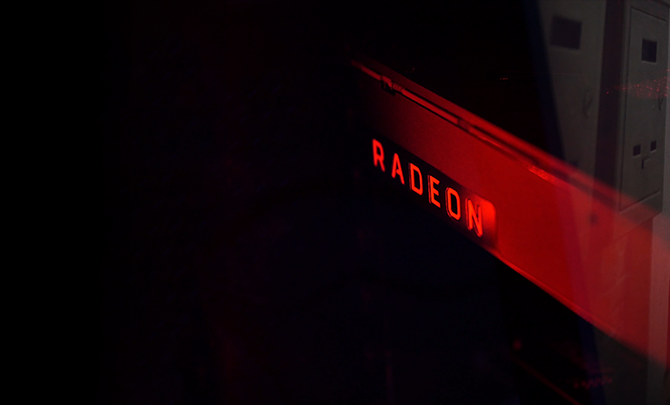
\includegraphics[width=\paperwidth,height=\paperheight]{gpu_background_black.png}
%% }
\pgfdeclareimage[width=\paperwidth]{mybackground}{gpu_background_black.png}
\setbeamertemplate{title page}{
  \begin{picture}(0,0)
    \put(-30,-163){%
      \pgfuseimage{mybackground}
    }
    \put(0,-150){%
      \begin{minipage}[b][45mm][t]{226mm}
        \usebeamerfont{title}{\inserttitle\par}
        \ifx\insertsubtitle\@empty%
        \else%
        {\vskip0.25em%
        \usebeamerfont{subtitle}\usebeamercolor[fg]{subtitle}\insertsubtitle\par}%
        \fi%
        \vskip1cm%              
        \usebeamerfont{author}{\insertauthor\par}
        \usebeamerfont{date}\url{malcolm.roberts@amd.com}\par
        \usebeamerfont{date}\insertdate
      \end{minipage}
    }
  \end{picture}
}

\setbeamerfont{frametitle}{family=\fontspec{Klavika-Regular.otf}}


%------------------------------------------------------------------------
%------------------------------------------------------------------------



\def\thetitle{rocFFT}
\def\thesubtitle{An open-source GPU FFT Library from AMD}
\def\theauthor{Malcolm Roberts}
\def\theauthorinstitute{AMD}

\def\presdate{2020-02-14}

\hypersetup{
  pdftitle=\thetitle{} \thesubtitle{},
  pdfauthor=\theauthor{}
}

\title{\thetitle{}}
\subtitle{\thesubtitle{}}
\author{\theauthor{}}
\institute{\theauthorinstitute}
%\date{\presdate}

\setbeamertemplate{frametitle}[default][center]
%\setbeamertemplate{footline}[frame number]
\setbeamertemplate{navigation symbols}{} 

\begin{document}

\klavikumfont

\setbeamertemplate{headline}{}
%\setbeamertemplate{footline}{}

{
  \setbeamercolor{background canvas}{bg=black}
  \setbeamercolor{normal text}{fg=white,bg=black}
  \setbeamercolor{frametitle}{fg=white}
  \setbeamercolor{title}{fg=white}
  \setbeamercolor{alerted text}{fg=white}
  \setbeamercolor{structure}{fg=white}
  \usebeamercolor[fg]{normal text}
  \begin{frame}
    \titlepage
  \end{frame}
}


\setbeamercolor{normal text}{fg=black,bg=white}
\usebeamercolor[fg]{normal text}

\newcolumntype{R}{>{\raggedleft\arraybackslash}X}
\setbeamertemplate{footline}{
   \leavevmode%
   \hbox{%
     \begin{beamercolorbox}[wd=\paperwidth,ht=1ex,dp=1.125ex]{author in head/foot}%
  \begin{tabularx}{\paperwidth}{lR}
    \hfill\insertframenumber/\inserttotalframenumber\hfill\phantom{.}%
    & %
    
\includegraphics[width=0.05\textwidth]{footerlogo}%
    \\%
  \end{tabularx}%
  \end{beamercolorbox}%
  }%
}

%% \begin{frame}
%%     \frametitle{Outline}
%%     \begin{itemize}
      
%%     \item ROCm: Radeon Open Compute Platform
%%     \item The \texttt{HIP} programming language
%%     \item \texttt{rocFFT}
%%       \begin{itemize}
%%         \item Design
%%         \item Features
%%         \item Usage
%%       \end{itemize}
%%     \item Sample applications
%%     \end{itemize}
      
%% \end{frame}

\begin{frame}
    \frametitle{ROCm\textsuperscript{\texttrademark}: Radeon Open Compute}

    \begin{center}
      \url{https://rocm.github.io/}
    \end{center}

    \begin{columns}
      \begin{column}{0.48\textwidth}
        \begin{itemize}
        \item Open source drivers and libraries
          \begin{itemize}
          \item Community engagement encouraged!
          \end{itemize}
        \item HPC and machine learning applications
        \item Focus on multi-gpu computation
        \item Some libraries of interest to the HPC community:
          \begin{itemize}
          \item rocBLAS
          \item rocSPARSE: sparse BLAS
          \item rocALUTION: sparse solvers
          \item rocFFT
          \end{itemize}
        \item Written in the HIP programming language
        \end{itemize}
      \end{column}
      \begin{column}{0.48\textwidth}
        
\includegraphics[width=0.9\textwidth]{ROCm-300x300.png}
      \end{column}
    \end{columns}
    
\end{frame}

\begin{frame}
    \frametitle{rocFFT: An open-source GPU FFT Library for Exascale Systems}

    \begin{center}
       \url{github.com/ROCmSoftwarePlatform/rocFFT}
    \end{center}

    \bigskip
    
    \begin{itemize}
    \item Open source
      \medskip
    \item Written in \texttt{C++}, \texttt{HIP}, and \texttt{Python}
      \medskip
    \item \texttt{rocfft} interface provides flexibility
      \medskip
    \item \texttt{hipfft} interface: usage similar to \texttt{cuFFT},
      calls either \texttt{rocFFT} or \texttt{cuFFT}
    \end{itemize}
    
\end{frame}

\begin{frame}
    \frametitle{rocFFT: design}

    \texttt{rocfft.h} provides a \texttt{C} interface.

    Based on the input parameters, we create a tree structure:
    \begin{itemize}
    \item Input and output buffers, strides, etc are assigned recursively.
    \item Leaf nodes contain device kernels.
    \item A plan is executed by traversing the leaf nodes sequentially.
    \end{itemize}

    \medskip
    
    Most kernels are generated.
    
    \medskip
    
    Kernel types:
    \begin{itemize}
    \item Stockham
    \item Transpose
    \item Bluestein
    \item Real/complex stages.
    \end{itemize}

\end{frame}

\begin{frame}
    \frametitle{rocFFT features}

    \begin{itemize}
    \item 1D, 2D, and 3D, transforms.
      \medskip
    \item Batched transforms.
      \medskip
    \item Single and double precision.
      \medskip
    \item In-place and out-of-place transforms.
      \medskip
    \item Input and output strides.
      \medskip
    \item Complex data format: interleaved or planar (aka ``split'').
      \medskip
    \item Extensive testing on several Linux distributions.
    \end{itemize}

\end{frame}

  
\begin{frame}
    \frametitle{rocFFT interface}

    \begin{center}
      The \texttt{rocfft} interface is defined in \texttt{rocfft.h}.
    \end{center}
    
    \begin{enumerate}
    \item \lstinline[]$rocfft_setup()$
    \item Optional: create a \lstinline[]$rocfft_plan_description$ for advanced stride and
      other format choices.
    \item Create a \lstinline[]$rocfft_plan$, possibly using the description above.
    \item Optional: Create a \lstinline[]$rocfft_execution_info$
      \begin{enumerate}
      \item Get the scratch memory requirements of the \lstinline[]$rocfft_plan$
      \item Allocate the work buffer and associate it to the \lstinline[]$rocfft_execution_info$
      \end{enumerate}
    \item Allocate the input and output buffers and set up the input data.
    \item Execute the plan with \lstinline[]$rocfft_execute$.
    \item Free the buffers, destroy the \texttt{rocFFT} structures, and
      \lstinline[]$rocfft_cleanup()$.
    \end{enumerate}

    \texttt{Fortran} interface: \url{https://github.com/ROCmSoftwarePlatform/hipfort}

\end{frame}

\begin{frame}[fragile]
    \frametitle{rocFFT: rocfft interface example}

\begin{lstlisting}
// Create the plan:
rocfft_plan gpu_plan = NULL;
rocfft_plan_create(&gpu_plan,    
                   rocfft_placement_inplace,
                   rocfft_transform_type_complex_forward,
                   rocfft_precision_double,
                   1,       // dimension
                   &length, // transform lengths (column-major)
                   1,       // batch size
                   NULL);   // optional description

std::complex<double>* gpu_in = NULL;
hipMalloc(&gpu_in, length[0] * sizeof(std::complex<double>));
                   
// Execute the plan:
rocfft_execute(gpu_plan, gpu_in, NULL, NULL);

// Destroy the plan:
hipFree(gpu_in);
rocfft_plan_destroy(gpu_plan);
\end{lstlisting}
\end{frame}
    
\begin{frame}
  \frametitle{hipFFT interface}
  \url{https://github.com/ROCmSoftwarePlatform/hipFFT}
  
  \texttt{hipFFT} Provides a \texttt{cuFFT}-like interface.

  \begin{itemize}
  \item \texttt{rocFFT} or \texttt{cuFFT} back-end.
  \item Row-major interface.
  \item Separate interfaces for 1D, 2D, and 3D.
  \item Work memory is handled internally.
  \item \texttt{Fortran} interfaces also available.
  \end{itemize}
  
\end{frame}
    
\begin{frame}[fragile]
    \frametitle{rocFFT: hipfft interface example}

\begin{lstlisting}
// Create the plan:
hipfftPlan1d(&plan,      // plan handle
             Nx,         // transform lengths
             HIPFFT_Z2Z, // transform type (HIPFFT_C2C for float)
             1);         // number of transforms
// Can also call hipfftPlanMany
             
// Work memory is automatically created and associated with the plan.

// Execute the plan:
hipfftExecZ2Z(plan, x, x, direction);
\end{lstlisting}

\end{frame}

\begin{frame}
  \frametitle{Sample code}

  Samples are available at
    \medskip
  \begin{itemize}
  \item \url{github.com/ROCmSoftwarePlatform/rocFFT/tree/develop/clients/samples}
    \medskip
  \item \url{github.com/ROCmSoftwarePlatform/hipFFT/tree/master/clients/samples}
  \end{itemize}
    
  
\end{frame}


\begin{frame}[fragile]
  \frametitle{Conclusion}

  \begin{center}
    rocFFT is:
  \end{center}
  \bigskip
  \begin{itemize}
  \item An open-source GPU FFT library from AMD
  \medskip
  \item Part of ROCm: the Radeon Open Compute Platform
  \medskip
  \item Uses the HIP programming language
  \medskip
  \item Will be used by a number of applications for exascale computing.
  \end{itemize}

  \bigskip
  \begin{center}
    \url{github.com/ROCmSoftwarePlatform/rocFFT}
  \end{center}
  
\end{frame}

\begin{frame}
  \textbf{Disclaimer}
  \medskip

  \fontsize{8pt}{8pt}\selectfont
  The information presented in this document is for informational
  purposes only and may contain technical inaccuracies, omissions, and
  typographical errors. The information contained herein is subject to
  change and may be rendered inaccurate for many reasons, including
  but not limited to product and roadmap changes, component and
  motherboard version changes, new model and/or product releases,
  product differences between differing manufacturers, software
  changes, BIOS flashes, firmware upgrades, or the like. Any computer
  system has risks of security vulnerabilities that cannot be
  completely prevented or mitigated.  AMD assumes no obligation to
  update or otherwise correct or revise this information. However, AMD
  reserves the right to revise this information and to make changes
  from time to time to the content hereof without obligation of AMD to
  notify any person of such revisions or changes.
  \medskip
 
  THIS INFORMATION IS PROVIDED ``AS IS''. AMD MAKES NO REPRESENTATIONS
  OR WARRANTIES WITH RESPECT TO THE CONTENTS HEREOF AND ASSUMES NO
  RESPONSIBILITY FOR ANY INACCURACIES, ERRORS, OR OMISSIONS THAT MAY
  APPEAR IN THIS INFORMATION. AMD SPECIFICALLY DISCLAIMS ANY IMPLIED
  WARRANTIES OF NON-INFRINGEMENT, MERCHANTABILITY, OR FITNESS FOR ANY
  PARTICULAR PURPOSE. IN NO EVENT WILL AMD BE LIABLE TO ANY PERSON FOR
  ANY RELIANCE, DIRECT, INDIRECT, SPECIAL, OR OTHER CONSEQUENTIAL
  DAMAGES ARISING FROM THE USE OF ANY INFORMATION CONTAINED HEREIN,
  EVEN IF AMD IS EXPRESSLY ADVISED OF THE POSSIBILITY OF SUCH DAMAGES.
  \medskip
    
  Third-party content is licensed to you directly by the third party
  that owns the content and is not licensed to you by AMD.  ALL LINKED
  THIRD-PARTY CONTENT IS PROVIDED “AS IS” WITHOUT A WARRANTY OF ANY
  KIND.  USE OF SUCH THIRD-PARTY CONTENT IS DONE AT YOUR SOLE
  DISCRETION AND UNDER NO CIRCUMSTANCES WILL AMD BE LIABLE TO YOU FOR
  ANY THIRD-PARTY CONTENT.  YOU ASSUME ALL RISK AND ARE SOLELY
  RESPONSIBLE FOR ANY DAMAGES THAT MAY ARISE FROM YOUR USE OF
  THIRD-PARTY CONTENT.
  \medskip

  ATTRIBUTION\\
  © 2021 Advanced Micro Devices, Inc. All rights
  reserved. AMD, the AMD Arrow logo, ROCm, Radeon, Radeon Instinct and
  combinations thereof are trademarks of Advanced Micro Devices,
  Inc. in the United States and/or other jurisdictions. Other names
  are for informational purposes only and may be trademarks of their
  respective owners.
  
\end{frame}
  

\end{document}
